%% Theory
% - how do neutrinos interact
\section{Neutrino interactions}
Neutrinos are studied by observing their interactions.
It is therefore essential to know our model's neutrino interactions.
This section aims to list the known neutrino interacions using Feynman diagrams\marginnote{A handy tool to describe particle interactions! \href{https://www.youtube.com/watch?v=jNNXD7fuE5E}{Watch Feynman explaining their functionality in a lecture series at the University of Auckland in 1979.}}, classify events into common energy ranges using the energy-momentum transfer and list the elastic and quasi-elastic scattering interactions of neutrinos and anti-neutrinos.

\subsection{Currents of the weak interaction}
Ignoring gravitational interactions, neutrinos are assumed to interact only under weak interactions.
Consequently the involved mediators are the massive $W^\pm$- and the $Z$-boson\marginnote{Massive bosons: 80GeV and 91GeV. The high mass of the mediators is the reason for the short range of the weak interaction.}, the mediators for \glspl{cc} and \glspl{nc}.

\begin{figure}
  \centering
  \vspace{1em}
  \begin{fmffile}{nc}
    \begin{fmfgraph*}(135,75)
      \fmfleft{i1,i2}
      \fmfright{o1,o2}
      \fmf{fermion}{i1,v1,o1}
      \fmf{phantom}{i2,v2,o2}
      \fmf{photon}{v1,v2}
      \fmflabel{$\nu$}{i1}
      \fmflabel{$\nu$}{o1}
      \fmflabel{$Z$}{v2}
    \end{fmfgraph*}
    \hspace*{2em}
    \begin{fmfgraph*}(135,75)
      \fmfleft{i1,i2}
      \fmfright{o1,o2}
      \fmf{fermion}{o1,v1,i1}
      \fmf{phantom}{i2,v2,o2}
      \fmf{photon}{v1,v2}
      \fmflabel{$\bar{\nu}$}{i1}
      \fmflabel{$\bar{\nu}$}{o1}
      \fmflabel{$Z$}{v2}
    \end{fmfgraph*}
  \end{fmffile}

  \vspace*{2em}

  \begin{fmffile}{cc}
    \begin{fmfgraph*}(135,75)
      \fmfleft{i1,i2}
      \fmfright{o1,o2}
      \fmf{fermion}{i1,v1,o1}
      \fmf{phantom}{i2,v2,o2}
      \fmf{photon}{v1,v2}
      \fmflabel{$\nu_l$}{i1}
      \fmflabel{$l$}{o1}
      \fmflabel{$W^+$}{v2}
    \end{fmfgraph*}
    \hspace*{2em}
    \begin{fmfgraph*}(135,75)
      \fmfleft{i1,i2}
      \fmfright{o1,o2}
      \fmf{fermion}{o1,v1,i1}
      \fmf{phantom}{i2,v2,o2}
      \fmf{photon}{v1,v2}
      \fmflabel{$\bar{\nu}_l$}{i1}
      \fmflabel{$\bar{l}$}{o1}
      \fmflabel{$W^-$}{v2}
    \end{fmfgraph*}
  \end{fmffile}
  \caption{%
    Feynman diagrams of (ftltbr) neutrino and anti-neutrino interacting with neutral and charged currents.
  }
  \label{fig:currents}
  \vspace{1em}
\end{figure}

For interactions mediated by a \gls{nc} the neutrino remains a neutrino and the anti-neutrino remains an anti-neutrino.
When a neutrino interacts with another particle mediated by a \gls{cc} the resulting particle is the neutrino's associated lepton.
Anti-neutrinos consequently become their associated anti-lepton.
Since the lepton and anti-lepton's charge differ, the currents -- and therefore the mediators -- need to differ as well.\marginnote{Due to conservation of charge.}
Figure \ref{fig:currents} displays the Feynman diagrams of these two interactions.

\subsection{Energy-momentum transfer and event classification}

The interactions can be classified using the energy-momentum transfer between the interacting particles.
Assuming we know the initial and final four-momenta of an interacting particle $p_i^\mu = (E_i, \vec{p}_i)$ and $p_f^\mu = (E_f, \vec{p}_f)$, then the momentum energy transfer is given by
\begin{equation*}
  q = p_i^\mu - p_f^\mu = (\Delta E, \Delta \vec{p}).
\end{equation*}

\begin{figure}
  \centering
  \vspace{1em}
  \begin{tikzpicture}
    \draw[->]         (-3,2) -- node (a) [label={above:$\vec{p}_i$}] {} (0,0);
    \draw[->]         (0,0)  -- node (b) [label={above:$\vec{p}_f$}] {} (2,1);
    \draw[->, dashed] (0,0)  -- node (c) [label={left:$\vec{q}$}] {} (1,-3);
  \end{tikzpicture}
  \hspace*{4em}
  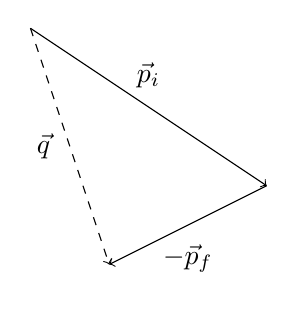
\begin{tikzpicture}
    \draw[->]         (-3,3) -- node (a) [label={above:$\vec{p}_i$}] {} (0,1);
    \draw[->]         (0,1)  -- node (b) [label={below:$-\vec{p}_f$}] {} (-2,0);
    \draw[->, dashed] (-3,3)  -- node (c) [label={left:$\vec{q}$}] {} (-2,0);
  \end{tikzpicture}
  \vspace{1em}
  \caption{%
    Illustration of the momentum transfer.
    $\vec{p}_i$ and $\vec{p}_f$ indicate the initial and final momenta.
    The image on the left shows the interaction of a classical particle transfering the momentum $\vec{q}$.
    If the momenta are rearranged like in the image on the right, it is obvious that $\vec{q}$ is given by $\vec{p}_i - \vec{p}_f$.
  }
  \label{fig:q}
\end{figure}

Given a flat Minkowski-space, the square of the norm of $q$ is given by
\begin{equation*}
  |q|^2 = (\Delta \vec{p})^2 - (\Delta E)^2,
\end{equation*}
where $\Delta E$ is the total transferred energy and $\Delta \vec{p}$ the total transferred momentum.
We can define how massive an event is\marginnote{See the analogy to $m^2 = E^2 - p^2$?}
\begin{align*}
  Q^2 &= (\Delta E)^2 - (\Delta \vec{p})^2 \\
      &= -q^2,
\end{align*}
and use this factor $Q^2$ to classify neutrino interaction events into:\\
\begin{tabular}{ l c }
  Elastic \& quasi-elastic scattering  & $Q^2 < 1 \text{GeV}^2$ \\
  Resonant scattering                  & $Q^2 \approx 1 \text{GeV}^2$ \\
  Deep inelastic scattering            & $Q^2 > 1 \text{GeV}^2$ \\
\end{tabular}

\subsection{Elastic \& quasi-elastic scattering} 
Interactions of $Q^2$ below 1GeV$^2$ are called elastic scattering events if they were mediated by the \gls{nc}.
Low energy scattering events mediated by \gls{cc} do not conserve kinetic energy, since part of it is needed to come up for the mass difference of the neutrino and its associated charged lepton.
For this reason these events are called quasi-elastic.
The terms \gls{ccqe} and \gls{nce} are commonly used to referr to these two classes of events.

If we list all possible interactions of neutrinos and anti-neutrinos with matter and anti-matter, we can see, that there's a clear symmetry in the case of the \gls{nce} -- see figure \ref{fig:elastic}.
The diagram for interactions of neutrinos with matter is equivalent to the diagram for the interactions of anti-neutrinos with anti-matter.
The same occurrs for interacions of neutrinos with anti-matter and anti-neutrinos with matter.

\begin{figure}
  \centering
  \vspace{1em}
  \begin{fmffile}{elastic}
    \begin{fmfgraph*}(135,75)
      \fmfleft{i1,i2}
      \fmfright{o1,o2}
      \fmf{fermion}{i1,v1,o1}
      \fmf{fermion}{i2,v2,o2}
      \fmf{photon,label=$Z$}{v1,v2}
      \fmflabel{$\nu_l$}{i1}
      \fmflabel{$q, l$}{i2}
      \fmflabel{$\nu_l$}{o1}
      \fmflabel{$q, l$}{o2}
    \end{fmfgraph*}
    \hspace*{2em}
    \begin{fmfgraph*}(135,75)
      \fmfleft{i1,i2}
      \fmfright{o1,o2}
      \fmf{fermion}{i1,v1,o1}
      \fmf{fermion}{o2,v2,i2}
      \fmf{photon,label=$Z$}{v1,v2}
      \fmflabel{$\nu_l$}{i1}
      \fmflabel{$\bar{q}, \bar{l}$}{i2}
      \fmflabel{$\nu_l$}{o1}
      \fmflabel{$\bar{q}, \bar{l}$}{o2}
    \end{fmfgraph*}

    \vspace*{4em}

    \begin{fmfgraph*}(135,75)
      \fmfleft{i1,i2}
      \fmfright{o1,o2}
      \fmf{fermion}{o1,v1,i1}
      \fmf{fermion}{i2,v2,o2}
      \fmf{photon,label=$Z$}{v1,v2}
      \fmflabel{$\bar{\nu}_l$}{i1}
      \fmflabel{$q, l$}{i2}
      \fmflabel{$\bar{\nu}_l$}{o1}
      \fmflabel{$q, l$}{o2}
    \end{fmfgraph*}
    \hspace*{2em}
    \begin{fmfgraph*}(135,75)
      \fmfleft{i1,i2}
      \fmfright{o1,o2}
      \fmf{fermion}{o1,v1,i1}
      \fmf{fermion}{o2,v2,i2}
      \fmf{photon,label=$Z$}{v1,v2}
      \fmflabel{$\bar{\nu}_l$}{i1}
      \fmflabel{$\bar{q}, \bar{l}$}{i2}
      \fmflabel{$\bar{\nu}_l$}{o1}
      \fmflabel{$\bar{q}, \bar{l}$}{o2}
    \end{fmfgraph*}
  \end{fmffile}
  \caption{%
    First order neutrino elastic scattering Feynman diagrams.
    $q$ stands for a quark of any flavor in a baryon, since quarks are not found free in nature.
    The diagram on the top left is equivalent to the diagram on the bottom right.
    The diagrams on the top right and the bottom left are equivalent as well.
  }
  \label{fig:elastic}
  \vspace{1em}
\end{figure}

\Gls{ccqe} lack such a symmetry, i.e. none of the four diagrams is equivalent -- see figure \ref{fig:quasielastic}.
Similar diagrams are found by changing the involved particles and mediators by their anti-particles and viceversa.

\begin{figure}
  \centering
  \vspace{1em}
  \begin{fmffile}{quasi}
    \begin{fmfgraph*}(135,75)
      \fmfleft{i1,i2}
      \fmfright{o1,o2}
      \fmf{fermion}{i1,v1,o1}
      \fmf{fermion}{i2,v2,o2}
      \fmf{photon,label=$W$}{v1,v2}
      \fmflabel{$\nu_l$}{i1}
      \fmflabel{$d, l$}{i2}
      \fmflabel{$l$}{o1}
      \fmflabel{$u, \nu$}{o2}
    \end{fmfgraph*}
    \hspace*{2em}
    \begin{fmfgraph*}(135,75)
      \fmfleft{i1,i2}
      \fmfright{o1,o2}
      \fmf{fermion}{i1,v1,o1}
      \fmf{fermion}{o2,v2,i2}
      \fmf{photon,label=$W$}{v1,v2}
      \fmflabel{$\nu_l$}{i1}
      \fmflabel{$\bar{u}$}{i2}
      \fmflabel{$l$}{o1}
      \fmflabel{$\bar{d}$}{o2}
    \end{fmfgraph*}

    \vspace*{4em}

    \begin{fmfgraph*}(135,75)
      \fmfleft{i1,i2}
      \fmfright{o1,o2}
      \fmf{fermion}{o1,v1,i1}
      \fmf{fermion}{i2,v2,o2}
      \fmf{photon,label=$W$}{v1,v2}
      \fmflabel{$\bar{\nu}_l$}{i1}
      \fmflabel{$u$}{i2}
      \fmflabel{$\bar{l}$}{o1}
      \fmflabel{$d$}{o2}
    \end{fmfgraph*}
    \hspace*{2em}
    \begin{fmfgraph*}(135,75)
      \fmfleft{i1,i2}
      \fmfright{o1,o2}
      \fmf{fermion}{o1,v1,i1}
      \fmf{fermion}{o2,v2,i2}
      \fmf{photon,label=$W$}{v1,v2}
      \fmflabel{$\bar{\nu}_l$}{i1}
      \fmflabel{$\bar{d}$, $\bar{l}$}{i2}
      \fmflabel{$\bar{l}$}{o1}
      \fmflabel{$\bar{u}$, $\bar{\nu}_l$}{o2}
    \end{fmfgraph*}
  \end{fmffile}
  \caption{%
    First order Feynman diagrams for quasielastic scattering.
    $u$ and $d$ stand for up-like and down-like quarks in a baryon.
    No equivalence can be found in these diagrams.
  }
  \label{fig:quasielastic}
  \vspace{1em}
\end{figure}

